% 论文地理空间图内嵌效果演示（geo.md 指导）：choropleth 比率 + 比例符号 + 小倍数
% 编译：xelatex -interaction=nonstopmode paper_embedded_geo.tex（两遍，交叉引用）
% fontset=none：禁止 ctex 自行选择 CJK 字体（它在 Linux 上会去找 Fandol 并可能失败），
% 中英文字体统一由下面的 \input{.../fonts-serif.tex} 决定（见 spec/type.md §1）
\documentclass[12pt,fontset=none]{ctexart}
\ctexset{fontset=none}
\usepackage[a4paper, margin=2.6cm]{geometry}
\usepackage{graphicx}
\usepackage{caption}
\captionsetup{font=small, labelsep=quad}
\setcounter{section}{2}
\renewcommand{\thefigure}{\thesection.\arabic{figure}}
% ============================================================
% pretty-charts 字体层：衬线搭配（宋体 + Times New Roman）
% 用法：\input{.../references/assets/tikz/fonts-serif.tex}
%
% 为什么单独成文件：示例此前各自写 \setmainfont{Times New Roman}
% + \setCJKmainfont{SimSun}，这两个字体只存在于 Windows，同一份示例在
% Linux/macOS 上无法编译（CI 也就无从编译）。这里按"字体是否存在"逐级回退：
%   Windows  → Times New Roman + SimSun（与原行为完全一致）
%   Linux    → TeX Gyre Termes + Noto Serif CJK SC（apt install fonts-noto-cjk-extra）
%   兜底     → TeX Gyre Termes + FandolSong（TeX Live 自带）
%   再兜底   → 只发警告、不设字体，保证编译不因缺字体而失败（中文可能显示异常）
% \IfFontExistsTF 由 fontspec 提供（preamble.tex 已加载 fontspec）。
% ============================================================
\IfFontExistsTF{Times New Roman}
  {\setmainfont{Times New Roman}}          % Windows / macOS
  {\IfFontExistsTF{TeX Gyre Termes}
     {\setmainfont{TeX Gyre Termes}}        % Linux 需 apt install fonts-texgyre
     {\PackageWarning{pretty-charts}{未找到西文衬线字体（Times New Roman / TeX Gyre %
       Termes），改用 XeLaTeX 默认西文字体；如需一致字形请安装 fonts-texgyre}}}
\IfFontExistsTF{SimSun}
  {\setCJKmainfont{SimSun}}                % 中文宋体（Windows）
  {\IfFontExistsTF{Noto Serif CJK SC}
     {\setCJKmainfont{Noto Serif CJK SC}}   % Linux（fonts-noto-cjk-extra）
     {\IfFontExistsTF{FandolSong}
        {\setCJKmainfont{FandolSong}}        % 兜底：TeX Live 自带，无需系统字体包
        {\PackageWarning{pretty-charts}{未找到中文衬线字体（已尝试 SimSun / %
          Noto Serif CJK SC / FandolSong）；中文可能显示异常。%
          请安装 fonts-noto-cjk-extra，或改用 fonts-sans.tex}}}}


\begin{document}
\section{系统设计与实现}

全球研发活动的空间分布高度不均衡。以每百万人口研发人员数衡量的投入强度在国家间相差
近百倍，而支出总额的绝对规模呈现另一番格局：美国与中国合计占全球研发支出的一半以上，
但人均强度并不突出。空间分布、绝对规模与两期演变分别如图~\ref{fig:choro}、
图~\ref{fig:bubble}~与图~\ref{fig:multiples}~所示。

\begin{figure}[htbp]
  \centering
  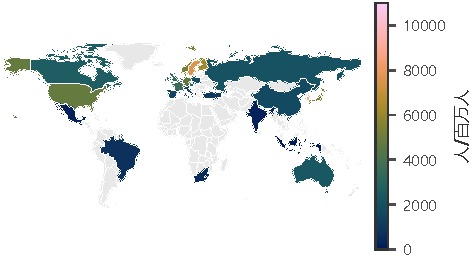
\includegraphics{fig1.pdf}
  \caption{各国研发人员密度（人/百万人）。等经纬（plate carrée）近似并作 1.15 倍纵向
  补偿，未接地图投影库；灰色区域为数据缺失，色图为
  Crameri \emph{Batlow} 感知均匀顺序色图（Crameri et al., 2020）。}
  \label{fig:choro}
\end{figure}

图~\ref{fig:choro}~采用分级统计地图（choropleth）表达比率指标：颜色编码
\emph{每百万人口}的相对强度而非绝对规模，避免国土面积与数值大小混淆；无数据的
国家以中性灰表示，与色标最低色严格区分。

\begin{figure}[htbp]
  \centering
  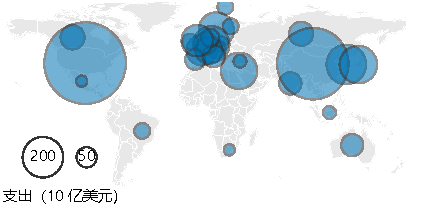
\includegraphics{fig2.pdf}
  \caption{各国研发支出总额（比例符号地图）。气泡面积与支出总额成正比，左下角
  为参照气泡（50 亿与 200 亿美元），半径按平方根定标。}
  \label{fig:bubble}
\end{figure}

与图~\ref{fig:choro}~互补，图~\ref{fig:bubble}~以比例符号表达支出总额这一绝对量：
气泡面积与数值成正比（半径为平方根），并提供参照气泡定标。比率用颜色、绝对量用
面积，两种编码各司其职，是空间数据可视化的基本分工。

\begin{figure}[htbp]
  \centering
  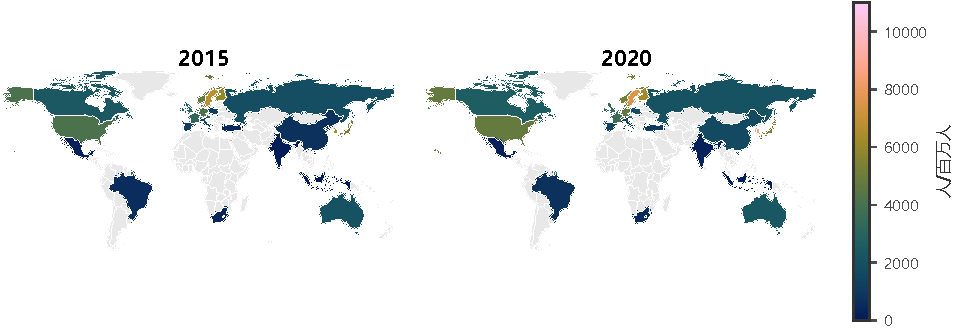
\includegraphics[width=\linewidth]{fig3.pdf}
  \caption{研发人员密度的两期对比（2015 与 2020）。两幅地图共享同一色标，可直接比较。}
  \label{fig:multiples}
\end{figure}

图~\ref{fig:multiples}~为两期小倍数对比：两幅地图共享同一色标范围，色块的深浅变化
即真实的时间变化；除中国、印度等少数国家外，多数国家的相对排位保持稳定。

\end{document}
